\documentclass[11pt]{article}

\usepackage[margin=1in]{geometry}
\usepackage{amsmath,amssymb,amsthm,mathtools}
\usepackage{booktabs,array}
\usepackage{graphicx}
\usepackage{microtype}
\usepackage{natbib}
\usepackage{setspace}
\usepackage{enumitem}
\usepackage[hidelinks]{hyperref}

\onehalfspacing
\setlength{\parindent}{1.4em}
\setlength{\parskip}{0pt}
\setlist[itemize]{leftmargin=1.6em,itemsep=2pt,topsep=3pt}
\setlist[enumerate]{leftmargin=1.8em,itemsep=2pt,topsep=3pt}

\newtheorem{proposition}{Proposition}
\newtheorem{corollary}{Corollary}
\newtheorem{lemma}{Lemma}
\theoremstyle{definition}
\newtheorem{definition}{Definition}
\theoremstyle{remark}
\newtheorem{remark}{Remark}

\newcommand{\LCA}{\ensuremath{\mathrm{LCA}}}
\newcommand{\Mcal}{\mathcal M}
\newcommand{\Rcal}{\mathcal R}

\title{\textbf{When Does Market Access Become Local Development?}\\
Platform Integration, Comparative-Advantage Realization,\\
and Local Value Capture}
\author{}
\date{July 2026}

\begin{document}

\maketitle

\begin{abstract}
\noindent
Platform integration can lower consumer prices everywhere without generating
local production and income everywhere.  This paper develops a tractable
theory of that divergence.  A platform simultaneously reallocates household
spending from a locally embedded channel toward an external channel and
expands the national market accessible to local producers.  New Structural
Economics disciplines the supply response: regional endowments determine
 latent comparative advantage; shared infrastructure determines whether an
 industry consistent with that advantage can cover all economic costs and
 enter; and a
fixed-cost--variable-cost choice determines whether production relies on an
external platform organization or becomes embedded in local complementary
services.  Payment flows, rather than an assumed local-capability index,
generate both consumer-channel retention and producer-side value capture.
The model yields four results.  Stronger latent comparative advantage lowers
the infrastructure thresholds for entry and local organizational
embeddedness.  Nominal and consumption-equivalent local income have distinct
infrastructure thresholds; the latter is weakly lower because consumers also
benefit from the price decline.  Government participation that relaxes a
shared-infrastructure financing constraint raises infrastructure supply and
 reduces the participation needed to cross those thresholds.  A separate
 external-channel restriction can also induce localization, but only by
 worsening the outside option, thereby reducing consumer access and possibly
 deterring marginal producers.  Illustrative numerical exercises establish
that the relevant parameter regions are nonempty; they are not a calibration.
\end{abstract}

\noindent\textit{Keywords:} platform integration; local value capture; latent
comparative advantage; organizational embeddedness; facilitating state;
regional development.

\noindent\textit{JEL codes:} F12, O14, O18, R11, L81.

\section{Introduction}

Digital platforms and domestic market integration can make a national market
look more uniform from the consumer's side.  A household in a remote place can
buy varieties previously available only in a large city, and the effective
price of those varieties falls as search, payment, and delivery improve.
Evidence from online trade in China shows that e-commerce reduces the role of
distance and disproportionately improves consumption access in smaller and
more remote cities \citep{FanTangZhuZou2018}.  Rural e-commerce expansion also
reduced the cost of living for adopters in the experiment studied by
\citet{CoutureFaberGuLiu2021}.  Similar consumer gains arise when modern retail
channels enter developing markets \citep{AtkinFaberGonzalezNavarro2018}.

Consumer access, however, is not the same object as local development.  The
rural e-commerce program studied by \citet{CoutureFaberGuLiu2021} produced
little average evidence of higher income for local producers and workers.
Modern retail entry can lower the cost of living while displacing income and
profits in incumbent local stores \citep{AtkinFaberGonzalezNavarro2018}.
More generally, reductions in domestic trade costs do not guarantee that
peripheral places industrialize: highway connections to larger markets
reduced industrial growth in the peripheral Chinese counties examined by
\citet{Faber2014}.  These findings are not evidence that integration is
generally harmful.  They show that an improvement in the set of goods a place
can buy need not coincide with an improvement in what that place can
competitively produce, organize, and retain.

This paper asks when platform-enabled market access becomes local development.
Its central distinction is between \emph{access} and \emph{capture}.  Access
describes the effective prices and market opportunities faced by local
consumers and producers.  Capture describes the location of the production,
service, and profit income generated by the associated transactions.  A
platform can improve inbound consumer access while shifting local expenditure
away from locally embedded wholesale, retail, logistics, and after-sales
services.  The same platform can improve outbound producer access, but a local
industry must still be sufficiently competitive to enter, and it may continue
to purchase marketing, fulfillment, certification, settlement, and supply
chain services from outside the region after entry.  Market participation
therefore admits an economically important intermediate state: local
production has been realized, but its organization remains externally
dependent.

New Structural Economics (NSE) supplies the production-side discipline needed
to explain this intermediate state.  NSE starts from the proposition that an
economy's industrial structure is conditioned by its endowment
structure and that each industrial structure requires corresponding hard and
soft infrastructure \citep{Lin2011,Lin2012}.  A firm in an industry consistent
with the comparative advantage implied by local factor endowments can
nevertheless fail to operate if transaction and coordination costs remain too
high.  \citet{LinWang2023} distinguish latent comparative advantage (LCA),
which is the specialization potential indicated by relative production costs,
from actual comparative advantage (ACA), which appears in realized production
and exports only after transaction costs are taken into account.  This paper
uses the domestic-market analogue of that distinction.  It does not introduce
a free-standing ACA index or treat ``realization'' as a third comparative-
advantage concept.  Instead, it asks the narrower equilibrium question required
by the platform problem: how much shared infrastructure is needed for an
LCA-consistent industry to enter the national market and then organize local
complementary services?  The policy distinction matters because shared
infrastructure constraints often cannot be removed by a single firm.  A
facilitating state can help industries with latent comparative advantage
overcome infrastructure and coordination constraints \citep{LinMonga2010}; it
is not meant to sustain indefinitely an industry that remains nonviable in open
competition \citep{Lin2003}.

The use of NSE here is deliberately narrower than a general theory of
structural transformation and broader than relabeling an exogenous
``capacity'' parameter.  Endowments determine relative production costs.
Infrastructure affects actual delivered costs and producer market access.
Those objects jointly determine whether the LCA-consistent industry is
actually produced and sold---the realization margin that
\citet{LinWang2023} associate with the movement from LCA to ACA.  The
organizational form used after entry then determines the location of
complementary-service payments.  Thus NSE affects both whether local
production exists and how much of the resulting value is locally embedded.
It does not replace consumer demand, the platform shock, or the local-income
propagation mechanism.

The model has five parts.  First, a representative household consumes a market
good through a local channel and an external platform channel.  Platform
integration lowers the platform price, raises its expenditure share, and
lowers the market-good price index.  The local income content of each channel
comes from a payment-flow table.  When the local channel has greater local
income content, the channel shift creates a consumer-side capture drag.

Second, a focal region is embedded in an otherwise exogenous national market.
A competitive background industry determines local factor opportunity costs.
The region's capital--labor endowment and the candidate industry's factor
intensity generate its unit production cost.  LCA is defined strictly as a
region--industry double relative production cost.  Transaction costs,
infrastructure, and market size then determine whether that latent cost
advantage is realized in equilibrium entry, production, and sales.  The
nonnegative-profit condition is consistent with \citet{Lin2003}'s viability
criterion because fixed costs include the owners' normal return and the model
does not use continuing selective protection.  Viability is not introduced as
another state variable or another threshold.

Third, a representative candidate producer faces CES national demand.  The
same platform-integration index that reduces the consumer platform price also
expands producer market access.  Shared infrastructure reduces outbound
iceberg costs.  A producer can rely on an external platform organization with
a low fixed cost and a high unit service payment, or build a locally embedded
organization with a higher fixed cost and a lower unit organizational cost.
This conditional fixed-cost--variable-cost ordering is related to the trade
intermediation mechanism in \citet{AhnKhandelwalWei2011}.  The interpretation
of embeddedness as locally supplied specialized producer services follows the
development-linkage logic of \citet{RodriguezClare1996}.  The present paper
uses only these two specific ingredients, not either paper's full model.

Fourth, the producer's revenue is split according to the location of actual
payments.  In the external mode, the unit platform-service payment leaves the
region.  In the local mode, production and complementary organizational
services are locally supplied.  These payment flows generate the
producer-retention rate; no separate retention-capacity function is assumed.
The resulting first-round producer income enters an EL-compatible
local-income propagation equation.  The propagation block is a one-region,
household-endogenous multiplier, closely related to standard social-accounting
and local-multiplier reasoning \citep{MillerBlair2009,Moretti2010}.  Its role
is conditional: it transmits first-round income generated by the new model
rather than constituting the new contribution.

Finally, a reduced-form infrastructure provider faces a financing wedge that
falls with government participation.  This is a narrow adaptation of the
financing mechanism in \citet{LinWang2023}, nested within the broader NSE
facilitating-state logic in \citet{Lin2011,Lin2012,LinMonga2010}: the state
helps relax a financing constraint on shared, transaction-cost-reducing
infrastructure.  It is not a national social planner, and the paper does not
claim that the chosen government participation is nationally optimal.

Four propositions organize the results.  Proposition~1 shows that stronger
LCA lowers the infrastructure required for profitable entry and actual
production.  Proposition~2 shows
that a second threshold determines organizational embeddedness; stronger LCA
also lowers this threshold, and crossing it changes local service income,
external payments, and the producer-retention rate.  Proposition~3 combines
these supply responses with the consumer channel shift.  It establishes
unique minimum infrastructure thresholds for nonnegative nominal and
consumption-equivalent income effects under endpoint-crossing conditions.
The real-income threshold is weakly below the nominal-income threshold and is
strictly below it when the two roots are interior to the same continuous
organizational regime.  This qualification matters because discrete entry or
organization switches can make the thresholds coincide.  Proposition~4 maps
the thresholds into minimum government-participation levels.  A separate
policy example contrasts cost-reducing facilitation with an
external-channel restriction.

The paper contributes to three literatures.  Relative to the literature on
e-commerce and retail access, it explains why consumer price gains can be more
geographically diffuse than producer and income gains.  Relative to NSE, it
introduces platform-mediated organizational dependence as a distinct stage
between realizing production and embedding complementary services locally.
Relative to local-multiplier models, it derives the first-round local-income
term and retention rates from comparative advantage, entry, organization, and
payment location.  The contribution is not the multiplier itself and not a
claim that local retention should be maximized at the expense of consumers.

A companion Economics Letters project in this research program takes
first-round producer income and channel retention as given and studies their
short-run propagation.  The present paper neither repeats that contribution
nor uses NSE merely to rename its exogenous local-capability parameter.
Instead, the new results are the endowment-based entry threshold, the
organizational-embeddedness threshold, and the payment flows that generate
first-round local producer income.  The multiplier is retained only to make
the two papers analytically compatible.

The analysis is intentionally a small-region partial equilibrium.  It does not
contain migration, land, endogenous national expenditure, platform strategic
pricing, or New Economic Geography agglomeration.  It therefore cannot
evaluate national welfare or long-run spatial equilibrium.  This restriction
keeps the paper focused on the question that motivates it: when a common
platform improves access, what structural conditions allow a region to
convert that opportunity into locally captured income?

\section{The Access--Capture Benchmark}

\subsection{Households and consumer access}

A representative household allocates nominal income among a market-good
composite \(Q_M\), a locally produced nontraded good \(N\), and an outside
numeraire \(Z\):
\begin{equation}
 U=Q_M^{\alpha_M}N^\beta Z^{1-\alpha_M-\beta},
 \qquad
 \alpha_M>0,\quad \beta\geq0,\quad \alpha_M+\beta<1.
 \label{eq:utility}
\end{equation}
Following the standard CES benchmark \citep{DixitStiglitz1977}, the market-good
composite is purchased through a locally embedded channel
\(A\) and an external platform channel \(P\):
\begin{equation}
 Q_M=
 \left[
 (1-a_P)^{1/\eta}Q_A^{(\eta-1)/\eta}
 +a_P^{1/\eta}Q_P^{(\eta-1)/\eta}
 \right]^{\eta/(\eta-1)},
 \qquad \eta>1.
 \label{eq:consumer_ces}
\end{equation}
Normalize \(p_A=1\).  Platform integration \(z\) lowers the effective platform
price:
\begin{equation}
 p_P(z)=\bar p_Pe^{-z}.
 \label{eq:platform_price}
\end{equation}
This price can include the delivered product price, search and payment costs,
and any consumer-facing platform charge.  It is distinct from the
producer-side organizational payment introduced below.

The platform expenditure share and market-good price index are:
\begin{align}
 s(z)
 &=
 \frac{a_Pp_P(z)^{1-\eta}}
 {(1-a_P)p_A^{1-\eta}+a_Pp_P(z)^{1-\eta}},
 \label{eq:platform_share}\\
 P_M(z)
 &=
 \left[
 (1-a_P)p_A^{1-\eta}
 +a_Pp_P(z)^{1-\eta}
 \right]^{1/(1-\eta)}.
 \label{eq:price_index}
\end{align}
Standard CES differentiation gives:
\begin{equation}
 s'(z)=(\eta-1)s(z)[1-s(z)]>0,
 \qquad
 \frac{d\ln P_M(z)}{dz}=-s(z)<0.
 \label{eq:consumer_comparative_static}
\end{equation}
Thus the platform unambiguously improves the model's consumer-access object:
its expenditure share rises and the cost of a unit of \(Q_M\) falls.

\subsection{Consumer-channel payment incidence}

Access does not determine where income is generated.  Let \(\ell_A\) and
\(\ell_P\) denote the local income generated per unit of expenditure through
the two consumer channels.  Table~\ref{tab:consumer_flows} clarifies their
content.  Both measures use the same transaction boundary and therefore can
be combined without treating an external payment as a national resource loss.
Formally, for \(r\in\{A,P\}\):
\begin{equation}
 \ell_r=\frac{LI_r}{E_r},
 \qquad 0\leq\ell_r\leq1.
 \label{eq:consumer_local_content_definition}
\end{equation}
Here \(E_r\) is gross local-household expenditure through channel \(r\), and
\(LI_r\) is the associated local factor income plus locally owned operating
surplus plus local service value added.
Taxes and transfers are excluded because the model contains no government
budget or interregional transfer rule.

\begin{table}[htbp]
\centering
\caption{Consumer-channel payment incidence}
\label{tab:consumer_flows}
\begin{tabular}{p{0.39\textwidth}cc}
\toprule
Payment generated by one unit of local household expenditure
& Local channel \(A\) & External platform \(P\)\\
\midrule
Local wholesale, retail, storage, and after-sales value added
& local income & limited in baseline\\
External production and interregional shipping
& external payment & external payment\\
Platform, settlement, and externally supplied digital services
& limited & external payment\\
Locally owned operating surplus
& local income & included if locally owned\\
\midrule
Local income content
& \(\ell_A\) & \(\ell_P\)\\
\bottomrule
\end{tabular}
\end{table}

The baseline assumes \(\ell_A>\ell_P\).  This is a transparent spatial
incidence assumption, not an assertion that platforms always retain less
value locally.  A platform that develops local fulfillment, seller services,
or ownership can have \(\ell_P\geq\ell_A\); that reverse case is reported in
the appendix.

The local income content of household market-good expenditure is:
\begin{equation}
 \omega_C(z)=[1-s(z)]\ell_A+s(z)\ell_P.
 \label{eq:consumer_retention}
\end{equation}
Define:
\begin{equation}
 D(z)=1-\beta-\alpha_M\omega_C(z).
 \label{eq:denominator}
\end{equation}
Because \(\omega_C(z)\leq1\) and \(\alpha_M+\beta<1\),
\(D(z)\geq1-\alpha_M-\beta>0\); no additional stability assumption is
required.  When
\(\ell_A>\ell_P\), platform substitution lowers \(\omega_C\) and raises
\(D\).  The corresponding proportional capture drag is:
\begin{equation}
 \Lambda(z)=
 \frac{\alpha_M(\ell_A-\ell_P)s'(z)}
 {D(z)}>0.
 \label{eq:capture_drag}
\end{equation}
The numerator records how rapidly expenditure moves toward the lower-retention
channel; the denominator captures repeated local spending.  This term is
consumer-side channel displacement.  It is separate from the producer-side
external platform payment developed in Section~\ref{sec:organization}.

\section{Endowments, Comparative Advantage, and Producer Access}

\subsection{A focal region and factor opportunity costs}

Consider a small focal region \(i\) with baseline factor endowments \(K_i\) and
\(L_i\).  Let:
\begin{equation}
 e_i=\frac{K_i}{L_i}.
 \label{eq:endowment_ratio}
\end{equation}
A competitive background industry \(0\) uses:
\begin{equation}
 Y_{i0}=A_0K_{i0}^{\theta_0}L_{i0}^{1-\theta_0}.
 \label{eq:background_technology}
\end{equation}
The candidate industry is small relative to the background economy.  The
background industry therefore determines the factor opportunity costs
relevant for its entry decision.  Over the range studied, marginal factor
services can be supplied at those opportunity costs without changing the
factor-price schedule.  This assumption can represent underused capacity,
additional work hours, or a locally elastic short-run supply margin.  With the
background good as numeraire, competitive factor pricing gives:
\begin{equation}
 w_i=(1-\theta_0)A_0e_i^{\theta_0},
 \qquad
 r_i=\theta_0A_0e_i^{\theta_0-1}.
 \label{eq:factor_prices}
\end{equation}
This closure avoids treating factor prices as free parameters while preserving
a tractable small-region problem.  It is not a full-employment two-sector
general equilibrium: a long-run welfare analysis would have to subtract
production forgone in the background industry and solve the factor
reallocation explicitly.

Candidate industry \(j\) uses:
\begin{equation}
 Y_{ij}=A_jK_{ij}^{\theta_j}L_{ij}^{1-\theta_j}.
 \label{eq:candidate_technology}
\end{equation}
Its unit production cost is:
\begin{align}
 c^P_{ij}
 &=
 \frac{1}{A_j}
 \left(\frac{r_i}{\theta_j}\right)^{\theta_j}
 \left(\frac{w_i}{1-\theta_j}\right)^{1-\theta_j}
 \notag\\
 &=\xi_j e_i^{\theta_0-\theta_j},
 \qquad \xi_j>0.
 \label{eq:unit_production_cost}
\end{align}
If the candidate industry is more capital intensive than the background
industry, \(\theta_j>\theta_0\), a higher regional capital--labor endowment
lowers its relative unit cost.  This is the minimal factor-proportions channel
required for an NSE paper.  It is consistent with the broader result that
factor abundance shifts production and trade toward industries intensive in
the abundant factor \citep{Romalis2004}, and with the NSE view that industrial
composition evolves with endowment structure \citep{JuLinWang2015}.

\subsection{Latent comparative advantage and actual realization}

The NSE sources do not posit a four-stage sequence consisting of separate LCA,
ACA, viability, and realization variables.  The distinction used by
\citet{LinWang2023} has two economic margins.  Relative production costs,
predicted by endowments and technology, identify an industry's LCA.  Actual
production and exports depend on total costs, including the fixed and variable
transaction costs affected by hard and soft infrastructure; the realized
production and export pattern is ACA.  In their empirical analysis, LCA is
proxied by the distance between national factor endowments and product factor
requirements, while ACA is observed through export participation and revealed
comparative advantage.  In their model, infrastructure changes transaction
costs and hence the set of active industries.  ACA and ``realization'' are
therefore not two additional concepts to be modelled separately.

\begin{definition}[Latent comparative advantage]
In the terminology of \citet{LinWang2023}, an industry has
latent comparative advantage when the location has a relative production-cost
advantage rooted in its endowment structure, before the transaction costs
that determine actual competitiveness are added.  This definition combines
the NSE proposition that endowment structure determines comparative advantage
\citep{Lin2011,Lin2012,JuLinWang2015} with the production-cost/transaction-cost
distinction in \citet{LinWang2023}.

Let \(h\) be an external reference region and \(0\) a background industry in
each region.  The present paper represents the relative-production-cost
criterion by:
\begin{equation}
 \mathcal C^P_{ij}
 =
 \frac{c^P_{ij}/c^P_{i0}}
 {c^P_{hj}/c^P_{h0}}.
 \label{eq:lca}
\end{equation}
Region \(i\) has LCA in industry \(j\) when
\(\mathcal C^P_{ij}<1\).
\end{definition}

Equation~\eqref{eq:lca} is this paper's two-region, two-industry
implementation of the comparative-cost criterion; it is not a formula quoted
from \citet{LinWang2023}.  The double comparison is necessary because a low
absolute cost or a positive accounting margin is not comparative advantage.
The factor-proportions mechanism behind the relative cost is consistent with
\citet{Romalis2004}, while the interpretation of that cost pattern as
endowment-conditioned industrial potential follows NSE.  In the analytical
and numerical comparative statics below,
\(c\equiv c^P_{ij}\) is only a monotone sufficient statistic for
\(\mathcal C^P_{ij}\), holding the reference-region and
background-industry ratios fixed:
\begin{equation}
 \frac{\partial c}{\partial\mathcal C^P_{ij}}>0.
 \label{eq:cost_lca_mapping}
\end{equation}
Lower \(c\) therefore means stronger LCA within the stated comparison, but the
underlying definition remains equation~\eqref{eq:lca}.

The model does not construct a second, free-standing ACA index.  Such an index
would require total costs and organizational alternatives for both the focal
and reference regions, objects that are unnecessary in a focal-region model.
Instead, infrastructure \(G\) changes the focal region's transaction costs and
producer access, and the producer problem determines whether the candidate
industry is actually active.  When
\[
\max\{\pi_P,\pi_L\}\geq0,
\]
the LCA-consistent industry enters, produces, and sells through an available
organization.  This event is the model's domestic-market counterpart of the
LCA-to-ACA realization in \citet{LinWang2023}; it is not a new definition of
comparative advantage.

The related concept of viability comes from a different NSE argument.
\citet{Lin2003} defines a normally managed firm as viable when it can earn a
socially acceptable normal profit in a free, open, and competitive market
without external subsidy or protection.  The nonnegative-profit entry
condition above is compatible with that criterion once fixed costs include
the owners' normal return and shared infrastructure is distinguished from
open-ended firm-specific support.  It is not a complete separate model of
viability, however, and the paper introduces neither a viability index nor a
viability threshold distinct from entry.

The theoretical mapping used below is therefore:
\[
\underbrace{(E_i,\theta_j)\longmapsto c^P_{ij}/c^P_{i0}}_{\mathrm{LCA}}
\quad+\quad
\underbrace{(G,\tau_O,\Mcal)}_{\text{realization constraints}}
\quad\Longrightarrow\quad
\underbrace{\max_{r\in\{P,L\}}\pi_r\geq0}_
{\text{actual production / ACA}}.
\]
Observed entry alone cannot identify the counterfactual production-cost
comparison required for LCA, but the model needs no intervening ACA or
viability state.  The formal threshold \(G_E\) below is simply the minimum
infrastructure level for actual entry.

\subsection{Producer market access}

The candidate producer faces a national CES demand schedule:
\begin{equation}
 q_r=\Mcal(z,G)p_r^{-\sigma},
 \qquad \sigma>1.
 \label{eq:producer_demand}
\end{equation}
Outbound iceberg costs are:
\begin{equation}
 \tau_O(z,G)=\bar\tau_O\exp[-\psi z-\gamma G],
 \qquad \bar\tau_O\geq1,\quad\psi>0,\quad\gamma>0.
 \label{eq:iceberg}
\end{equation}
Here \(z\) lowers platform-mediated search, coordination, and delivery costs,
while \(G\) is common, non-firm-specific hard or soft infrastructure such as a
transport link, broadband backbone, public standard, certification system, or
contract-enforcement facility.  The local analysis is restricted to the range
in which the iceberg representation remains at least one.

Substituting equation~\eqref{eq:iceberg} into CES demand and absorbing the
invariant factor \(\bar\tau_O^{1-\sigma}\) and national expenditure into
\(\Mcal_0\) gives:
\begin{equation}
 \Mcal(z,G)
 =
 \Mcal_0
 \exp\left\{
 (\sigma-1)(\psi z+\gamma G)
 \right\}.
 \label{eq:market_access}
\end{equation}
This is the standard market-access mapping in which iceberg trade costs enter
CES demand with elasticity \(1-\sigma\)
\citep{DonaldsonHornbeck2016}.  The baseline deliberately excludes a direct
\(zG\) complementarity: both reforms lower the same outbound cost, and no
additional parameter is needed for the core results.  The appendix considers
the extension
\(\tau_O=\bar\tau_O\exp[-\psi z-\gamma G-\chi^{\mathrm{ext}}zG]\),
\(\chi^{\mathrm{ext}}>0\).

Equation~\eqref{eq:market_access} is not the consumer price equation written
twice.  Consumer access in equation~\eqref{eq:platform_price} concerns what
local households can buy; producer access concerns the demand that local
producers can reach.  The same platform reform \(z\) moves both, which keeps
the EL question intact, but the two margins have different payment incidence
and only producer access depends on \(G\).

\subsection{Entry and the actual-entry threshold}

The producer can use an external platform organization \(P\) or a locally
embedded organization \(L\):
\begin{equation}
 m_P=c+d_P,\qquad
 m_L=c+d_L,\qquad
 0\leq d_L<d_P,
 \label{eq:marginal_costs}
\end{equation}
\begin{equation}
 F_P=f,\qquad F_L=f+F,\qquad f>0,\quad F>0.
 \label{eq:fixed_costs}
\end{equation}
The external organization uses a platform's existing national marketing,
settlement, fulfillment, and supply-chain system.  It therefore avoids the
organization-specific fixed cost \(F\), but it entails a larger unit service
payment.  The common entry cost \(f\) is a private economic cost of product
adaptation, certification, and initial market entry; it includes the normal
return required for a zero-economic-profit entry boundary.  The additional
\(F\) is the private or
collectively financed setup cost of a local warehouse, operations team,
quality-control system, or seller-service network.  It is distinct from
\(G\), which is non-firm-specific shared infrastructure.  The local
organization builds or coordinates the complementary services represented by
\(F\) locally.  This ordering is conditional, not a universal property of
digital platforms.  It isolates a single organizational choice: buy an
external service flow or incur a fixed setup cost to embed that service
locally.

With constant elasticity demand, the markup, price, revenue, and profit are:
\begin{align}
 \mu&=\frac{\sigma}{\sigma-1},&
 p_r&=\mu m_r,
 \label{eq:markup}\\
 \Rcal_r(z,G)
 &=\Mcal(z,G)\mu^{1-\sigma}m_r^{1-\sigma},&
 \pi_r(z,G)
 &=\frac{\Rcal_r(z,G)}{\sigma}-F_r.
 \label{eq:revenue_profit}
\end{align}
The producer selects:
\begin{equation}
 r^*(z,G)\in\arg\max\{0,\pi_P(z,G),\pi_L(z,G)\}.
 \label{eq:producer_choice}
\end{equation}

Define:
\begin{equation}
 k=\frac{\mu^{1-\sigma}}{\sigma},
 \qquad
 \Omega=(\sigma-1)\gamma>0.
 \label{eq:k_omega}
\end{equation}
The zero-profit infrastructure threshold for organization \(r\) is:
\begin{equation}
 G_r^0(z,c)
 =
 \frac{
 \ln\left[
 \dfrac{F_r}
 {k\Mcal_0e^{(\sigma-1)\psi z}(c+d_r)^{1-\sigma}}
 \right]
 }{\Omega}.
 \label{eq:mode_entry_threshold}
\end{equation}
The economically relevant entry threshold is:
\begin{equation}
 G_E(z,c)=
 \max\left\{0,\min[G_P^0(z,c),G_L^0(z,c)]\right\}.
 \label{eq:entry_threshold}
\end{equation}

\begin{proposition}[LCA and actual entry]
\label{prop:entry}
Suppose \(\gamma>0\).  The minimum infrastructure level \(G_E\) for profitable
entry exists.  At an interior threshold:
\begin{equation}
 \frac{\partial G_E}{\partial c}>0,
 \qquad
\frac{\partial G_E}{\partial\mathcal C^P_{ij}}>0.
\label{eq:entry_lca_comparative_static}
\end{equation}
Hence stronger LCA lowers the shared infrastructure required for profitable
entry and actual production.  If a raw threshold is negative, its economically
truncated value is zero and the comparative static is weak.
\end{proposition}

The result is not an assumption that LCA raises local income.  It follows from
the profit problem: a lower endowment-conditioned production cost raises
operating profit under either organization and reduces the amount of
transaction-cost-reducing infrastructure needed to cover the fixed cost.
Proofs of all propositions are in the appendix.

\section{Organization, Capture, and Local Income}
\label{sec:organization}

\subsection{The organizational-embeddedness threshold}

The local mode has a higher operating-profit coefficient because
\(d_L<d_P\), but it must cover the additional fixed cost \(F\).  The
infrastructure level at which \(\pi_L=\pi_P\) is:
\begin{equation}
 G_X(z,c)
 =
 \frac{
 \ln\left[
 \dfrac{F}
 {k\Mcal_0e^{(\sigma-1)\psi z}
  \{(c+d_L)^{1-\sigma}-(c+d_P)^{1-\sigma}\}}
 \right]
 }{\Omega}.
 \label{eq:switch_threshold_raw}
\end{equation}
The economically relevant embeddedness threshold is defined directly from the
equilibrium choice:
\begin{equation}
 G_L(z,c)
 =
 \inf\left\{
 G\geq0:
 \pi_L(z,G)\geq\max\{0,\pi_P(z,G)\}
 \right\}.
 \label{eq:embedding_threshold}
\end{equation}

The full state classification requires distinguishing \(G_P^0\),
\(G_L^0\), and \(G_X\).  Let:
\begin{equation}
 b_r=k(c+d_r)^{1-\sigma},
 \qquad
 \bar F=f\frac{b_L-b_P}{b_P}.
 \label{eq:Fbar}
\end{equation}
If \(F>\bar F\), then:
\begin{equation}
 G_P^0<G_L^0<G_X.
 \label{eq:three_region_order}
\end{equation}
The equilibrium consequently passes through three regions as infrastructure
rises:
\[
\text{no entry}
\quad\longrightarrow\quad
\text{external platform dependence}
\quad\longrightarrow\quad
\text{local organizational embeddedness}.
\]
If \(F\leq\bar F\), the platform-dependent middle region can disappear:
the producer may move directly from no entry to the local organization.  The
middle state is therefore an economic result with a transparent parameter
condition, not a stage imposed by terminology.
Equivalently:
\begin{equation}
 G_L(z,c)
 =
 \begin{cases}
 \max\{0,G_X(z,c)\},&F>\bar F,\\
 \max\{0,G_L^0(z,c)\},&F\leq\bar F.
 \end{cases}
 \label{eq:embedding_threshold_piecewise}
\end{equation}

\subsection{Producer-side payment incidence}

Producer revenue is not automatically local income.  Let \(d_Pq_P\) be the
payment to the external platform and externally supplied complementary
services.  Production factors and the residual operating surplus are locally
owned in the baseline; imported intermediate inputs and outside equity are
excluded from the polar benchmark.  Under the local mode, the
organizational-service payment \(d_Lq_L\) is made to local providers.
Table~\ref{tab:producer_flows} records the incidence.

\begin{table}[htbp]
\centering
\caption{Producer organization and spatial payment incidence}
\label{tab:producer_flows}
\begin{tabular}{p{0.39\textwidth}cc}
\toprule
Payment generated by candidate-industry sales
& External mode \(P\) & Local mode \(L\)\\
\midrule
Local production-factor income
& local & local\\
Local producer operating surplus
& local & local\\
Unit marketing, settlement, fulfillment, and supply-chain service
& external \(d_Pq_P\) & local \(d_Lq_L\)\\
Shared organizational fixed cost
& not incurred & locally supplied \(F\)\\
Common entry cost
& locally supplied \(f\) & locally supplied \(f\)\\
\midrule
External payment included in retention measure
& \(d_Pq_P\) & \(0\)\\
\bottomrule
\end{tabular}
\end{table}

Fixed costs affect entry and organization, but locally supplied fixed-cost
services are payments to local factors or firms.  Deducting them again from
local income would double count a local resource payment.  Conversely, the
external unit payment is excluded from local income even if it is not a
national loss.  Equivalently, first-round local income is local factor income
plus locally owned operating surplus plus locally supplied producer-service
value added, all measured within the same transaction boundary.

Let \(B_j^r\) denote first-round local income generated by candidate-industry
sales:
\begin{equation}
 B_j^r(z,G)=\rho_r\Rcal_r(z,G).
 \label{eq:producer_local_income}
\end{equation}
The payment table implies:
\begin{equation}
 \rho_P
 =
 1-\frac{d_P}{\mu(c+d_P)}
 <1,
 \qquad
 \rho_L=1.
 \label{eq:producer_retention}
\end{equation}
The value \(\rho_L=1\) is a polar incidence benchmark, not a claim that every
locally organized supply chain has no outside payment.  It follows here from
local ownership of production and organizational services and the exclusion
of imported intermediates.  Allowing such payments would lower \(\rho_L\)
without changing the threshold logic provided the local mode remains more
locally embedded than the external mode.
If a fraction \(\lambda\in[0,1]\) of platform services is supplied locally:
\begin{equation}
 \rho_P(\lambda)
 =
 1-\frac{(1-\lambda)d_P}{\mu(c+d_P)}.
 \label{eq:partial_localization}
\end{equation}
The baseline is \(\lambda=0\).  This robustness parameter changes payment
location, not productive efficiency.

\begin{proposition}[Organizational embeddedness]
\label{prop:embedding}
Suppose \(d_L<d_P\), \(F>0\), and \(\Omega>0\).  There exists a
minimum embeddedness threshold \(G_L\).  At an interior threshold:
\begin{equation}
 \frac{\partial G_L}{\partial c}>0,
 \qquad
 \frac{\partial G_L}{\partial\mathcal C^P_{ij}}>0.
 \label{eq:embedding_lca}
\end{equation}
For \(G\geq G_L\), the producer selects \(L\), and the switch satisfies:
\begin{equation}
 \rho_L>\rho_P,\qquad
 \Rcal_L>\Rcal_P,\qquad
 B_j^L>B_j^P.
 \label{eq:embedding_capture}
\end{equation}
If \(F>\bar F\), platform dependence is a distinct equilibrium region between
entry and local embeddedness.  If \(F\leq\bar F\), that region may disappear.
\end{proposition}

This proposition is the main way NSE affects capture beyond production.
Stronger LCA makes local sales sufficiently large to cover the shared
organizational fixed cost at a lower infrastructure level.  Crossing the
threshold does not merely relabel the firm: it reduces external payments and
creates local complementary-service income.

\subsection{Nominal and consumption-equivalent local income}

Let \(B_0>0\) denote autonomous first-round income from the background economy
over the local partial-equilibrium range.  Consistent with the locally elastic
factor-supply assumption above, candidate-industry factor payments are
incremental nominal receipts; their full opportunity cost is not a welfare
gain.  Household spending generates additional rounds of local income.  The share \(\beta\)
spent on locally produced nontraded goods remains local.  The share
\(\alpha_M\) spent on market goods generates local income at rate
\(\omega_C(z)\).  Avoiding any duplication of the first-round producer
payments, nominal local income satisfies:
\begin{equation}
 Y=
 B_0+B_j^{r^*}(z,G)
 +\beta Y+\alpha_M\omega_C(z)Y.
 \label{eq:income_fixed_point}
\end{equation}
Therefore:
\begin{equation}
 Y(z,G)=
 \frac{B_0+B_j^{r^*}(z,G)}
 {D(z)}.
 \label{eq:nominal_income}
\end{equation}
This is a conditional local-income accounting equilibrium.  It is appropriate
when the relevant local services and nontraded goods can respond at a fixed
short-run opportunity cost.  It is not a full welfare measure.

Consumption-equivalent income deflates nominal income by the market-good price
index:
\begin{equation}
 R(z,G)=\frac{Y(z,G)}{P_M(z)^{\alpha_M}}.
 \label{eq:real_income}
\end{equation}
Define the candidate industry's share in first-round local income:
\begin{equation}
 \zeta_r(z,G)=
 \frac{B_j^r(z,G)}
 {B_0+B_j^r(z,G)}.
 \label{eq:zeta}
\end{equation}
Within a fixed organizational state, equations
\eqref{eq:market_access}, \eqref{eq:capture_drag}, and
\eqref{eq:nominal_income} yield:
\begin{equation}
 \frac{d\ln Y}{dz}
 =
 \zeta_r(z,G)(\sigma-1)\psi
 -\Lambda(z).
 \label{eq:nominal_effect}
\end{equation}
The first term is the local producer-income gain from better platform access.
Its direct elasticity \((\sigma-1)\psi\) is common across regions, but its
local-income effect is larger when infrastructure has already raised the
candidate industry's share \(\zeta_r\).  The second term is the
consumer-channel capture drag.

The consumption-equivalent effect is:
\begin{equation}
 \frac{d\ln R}{dz}
 =
 \frac{d\ln Y}{dz}
 +\alpha_Ms(z).
 \label{eq:real_effect}
\end{equation}
The final term is the direct consumer price benefit.  Equations
\eqref{eq:nominal_effect} and \eqref{eq:real_effect} preserve the original
access--capture question while replacing an exogenous producer gain and
retention capacity with equilibrium entry, organization, and payment flows.

\begin{proposition}[Nominal and real-income thresholds]
\label{prop:income_thresholds}
Suppose \(\psi>0\) and maintain the baseline payment ordering.  Within
each active producer organization, both \(d\ln Y/dz\) and \(d\ln R/dz\) are
strictly increasing in \(G\); in the no-entry state they are constant in
\(G\).  Entry and the switch from \(P\) to \(L\) generate upward jumps.  If
the relevant effect is negative at the lower endpoint and positive at an
upper endpoint, there is a unique minimum threshold:
\begin{align}
 G_Y&=\inf\left\{G:\frac{d\ln Y}{dz}\geq0\right\},
 \label{eq:GY}\\
 G_R&=\inf\left\{G:\frac{d\ln R}{dz}\geq0\right\}.
 \label{eq:GR}
\end{align}
Pointwise,
\begin{equation}
 G_R\leq G_Y.
 \label{eq:weak_order}
\end{equation}
If both roots are interior to the same continuous organizational region,
\begin{equation}
 G_R<G_Y.
 \label{eq:strict_order}
\end{equation}
If both effects cross zero at the same discrete entry or organization switch,
the thresholds can coincide.  Stronger LCA weakly lowers both thresholds and
strictly lowers them when the relevant roots remain interior to the same
organizational states.
\end{proposition}

In the unbounded-\(G\) baseline, sufficient upper-endpoint conditions are
\((\sigma-1)\psi>\Lambda(z)\) for the nominal threshold and
\((\sigma-1)\psi+\alpha_Ms(z)>\Lambda(z)\) for the real threshold.  These
conditions are substantive: after removing the unnecessary \(zG\) interaction,
the existence of a favorable high-infrastructure endpoint is no longer built
into the functional form.

The proposition separates three regional outcomes.  Below \(G_R\), producer
gains are too small to offset both channel displacement and the relevant cost
of living, so nominal and consumption-equivalent income fall.  Between
\(G_R\) and \(G_Y\), nominal income falls but the consumer price gain is large
enough to raise consumption-equivalent income.  Above \(G_Y\), producer access
and local capture are strong enough for both measures to rise.  The
classification is conditional: if \(\ell_P\geq\ell_A\), capture drag is
nonpositive and the low-infrastructure loss region can disappear.

\section{The Facilitating State}

\subsection{Infrastructure supply}

The preceding analysis treats \(G\) as a local structural condition.  This
section endogenizes its supply without introducing a national social planner.
Let \(\vartheta\in[0,1]\) denote government participation in infrastructure
finance.  The financing wedge is:
\begin{equation}
 \kappa_I(\vartheta)
 =
 \kappa_p-(\kappa_p-\kappa_g)\vartheta,
 \qquad
 0<\kappa_g<\kappa_p.
 \label{eq:financing_wedge}
\end{equation}
The infrastructure provider solves:
\begin{equation}
 \max_{G\geq0}
 \left\{
 \mathcal U_I(G)-\kappa_I(\vartheta)C(G)
 \right\},
 \label{eq:provider_problem}
\end{equation}
where:
\begin{equation}
 \mathcal U_I'>0,\quad
 \mathcal U_I''<0,\quad
 C'>0,\quad C''\geq0.
 \label{eq:provider_curvature}
\end{equation}
\(\mathcal U_I\) is the provider's appropriable revenue from infrastructure
services.  The gap between this revenue and the broader producer-access gains
captures the shared nature of logistics, standards, certification, digital
systems, and other infrastructure.  Government participation lowers the
financing wedge; it does not directly subsidize candidate-industry output.

An interior solution satisfies:
\begin{equation}
 \mathcal U_I'[G(\vartheta)]
 =
 \kappa_I(\vartheta)C'[G(\vartheta)].
 \label{eq:provider_foc}
\end{equation}
The curvature assumptions guarantee uniqueness.

\subsection{Government-participation thresholds}

\begin{proposition}[Government participation and threshold crossing]
\label{prop:state}
The infrastructure supply in equation~\eqref{eq:provider_problem} is unique
and:
\begin{equation}
 G'(\vartheta)>0.
 \label{eq:state_G}
\end{equation}
For \(H\in\{E,L,R,Y\}\), define the minimum government participation needed
to cross an existing threshold:
\begin{equation}
 \vartheta_H=\inf\{\vartheta:G(\vartheta)\geq G_H\}.
 \label{eq:state_thresholds}
\end{equation}
Greater government participation reduces each gap \(G_H-G(\vartheta)\).
Stronger LCA weakly lowers
\(\vartheta_E,\vartheta_L,\vartheta_R\), and \(\vartheta_Y\),
with strict effects where the corresponding structural thresholds are
interior.
\end{proposition}

\subsection{Cost-reducing facilitation versus an external-channel restriction}

The preceding proposition concerns only the supply of shared infrastructure.
It should not be read as a theorem that every state intervention is
facilitating.  To make the distinction concrete, consider a narrow
external-channel restriction that multiplies \(p_P\) by a wedge
\(\tau_C>1\) and raises \(d_P\).  This is not a general definition of
protection in NSE; it is a policy example tailored to the two channels in this
model.  The consumer price index rises and the platform expenditure share
falls.  On the producer side:
\begin{equation}
 \frac{\partial G_P^0}{\partial d_P}
 =
 \frac{\sigma-1}{\Omega(c+d_P)}>0.
 \label{eq:restriction_entry}
\end{equation}
The restriction therefore makes external-platform entry harder.  At the same
time, raising \(d_P\) increases the local mode's variable-cost advantage and
can lower \(G_X\).  It can induce localization by degrading the alternative.
Facilitation instead allows the region to cross the entry and embeddedness
thresholds by reducing a real shared constraint.  This conditional comparison
is consistent with the NSE distinction between facilitating an
LCA-consistent, potentially viable industry and protecting a nonviable
activity; it is not a complete ranking of all possible protection and
facilitation policies.

The state result is deliberately limited.  It does not prove that more
government participation is always desirable, that the provider captures all
social returns, or that \(\vartheta=1\) is optimal.  A complete national
welfare problem would require government fiscal costs, external platform
profits, other regions, and general-equilibrium factor responses, all of which
are outside the focal-region model.

\section{Illustrative Numerical Exercises}

\subsection{Purpose and parameterization}

The numerical exercises have one purpose: to demonstrate that the parameter
regions described by Propositions~\ref{prop:entry}--\ref{prop:state} are
nonempty and to display the model's discontinuities.  They are not a
calibration and none of the values is presented as an estimate for China.
Table~\ref{tab:parameters} reports the standardized baseline.

\begin{table}[htbp]
\centering
\caption{Illustrative baseline parameters}
\label{tab:parameters}
\begin{tabular}{lll}
\toprule
Block & Parameters & Values\\
\midrule
Household
& \(\alpha_M,\beta,\eta\)
& \(0.35,\ 0.30,\ 6\)\\
Consumer channels
& \(\ell_A,\ell_P,B_0\)
& \(0.70,\ 0.10,\ 1\)\\
Producer demand
& \(\sigma,\Mcal_0,\psi\)
& \(4,\ 5,\ 0.19\)\\
Infrastructure access
& \(\gamma\)
& \(0.10\)\\
Production and organization
& \(c,d_P,d_L,f,F\)
& \(0.9,\ 0.4,\ 0.1,\ 0.34,\ 0.53\)\\
State block
& \(\kappa_p,\kappa_g,a_I\)
& \(4.0,\ 0.30,\ 0.80\)\\
\bottomrule
\end{tabular}
\end{table}

The consumer CES weight is \(a_P=0.4\), and the pre-integration platform
price is \(\bar p_P=1.2\).  For the state exercise:
\begin{equation}
 \mathcal U_I(G)=a_I\ln(1+G),
 \qquad
 C(G)=\frac{G^2}{2}.
 \label{eq:numerical_state}
\end{equation}
Equation~\eqref{eq:provider_foc} then has the closed-form solution:
\begin{equation}
 G(\vartheta)=
 \frac{-1+\sqrt{1+4a_I/\kappa_I(\vartheta)}}{2}.
 \label{eq:numerical_G}
\end{equation}

\subsection{The structural phase diagram}

Figure~\ref{fig:phase} varies the candidate industry's relative production
cost and infrastructure at \(z=0.5\).  Moving right weakens LCA.  Moving up
improves the infrastructure through which LCA can be converted into actual
entry and local organization.  The colored regions are filled directly
between the analytical boundaries \(G_E(c)\) and \(G_L(c)\); they are not a
smoothed or interpolated classification grid.

\begin{figure}[htbp]
\centering
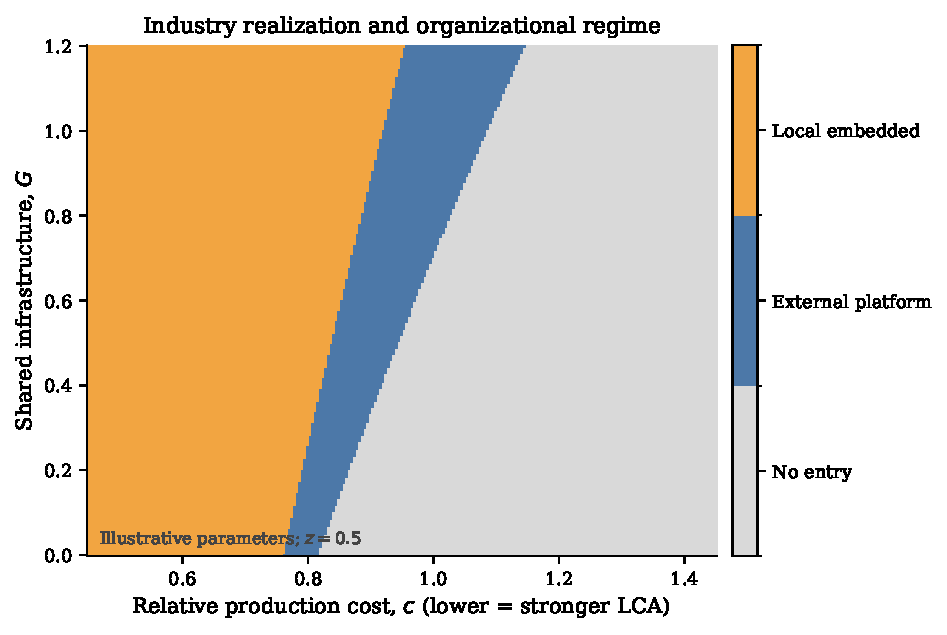
\includegraphics[width=0.78\textwidth]{../figures/figure_1_phase_diagram.pdf}
\caption{Analytical phase diagram for actual production and organization}
\label{fig:phase}
\end{figure}

The gray region contains no active candidate industry.  The blue region
contains local production that reaches the national market through the
external platform organization.  The orange region contains locally embedded
production and complementary services.  At a given \(G\), a stronger LCA
industry is more likely both to enter and to embed.  For an intermediate range
of production costs, increasing infrastructure moves the region through all
three states; sufficiently strong LCA can make the industry locally embedded
even at low \(G\), whereas sufficiently weak LCA may leave it unprofitable
throughout the plotted range.  The platform-dependent middle region is sizable
under the baseline because \(F>\bar F\); it is generated by the profit and
organization problem rather than imposed as an additional comparative-
advantage category.

\subsection{Infrastructure thresholds}

Figure~\ref{fig:thresholds} separates the structural and income thresholds
that were previously superimposed in one panel.  Panel (a) plots actual entry
and local embeddedness; its shaded band is the platform-dependent interval.
Panel (b) plots the real- and nominal-income thresholds; its shaded band is
the range in which the real effect is nonnegative but the nominal effect
remains negative.  All curves are computed from the exact equilibrium choice
and the minimum-\(G\) definitions in equations
\eqref{eq:entry_threshold}, \eqref{eq:embedding_threshold},
\eqref{eq:GY}, and \eqref{eq:GR}.

\begin{figure}[htbp]
\centering
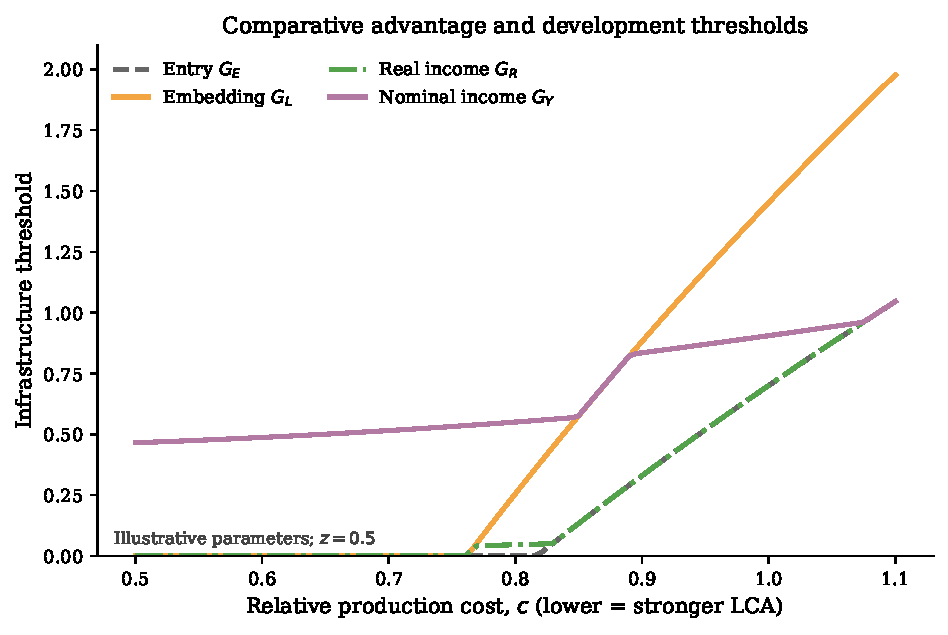
\includegraphics[width=\textwidth]{../figures/figure_2_thresholds.pdf}
\caption{LCA-conditioned infrastructure thresholds}
\label{fig:thresholds}
\end{figure}

All four thresholds weakly rise as LCA weakens.  Flat zero segments and kinks
are economically meaningful: they arise from the nonnegativity bound on
infrastructure or from a change in the active equilibrium mode.  They have
not been removed by statistical smoothing.  In the baseline at
\(c=0.9,z=0.5\), the relevant thresholds are:
\[
G_E=G_R=0.2106,\qquad
G_Y=0.5554,\qquad
G_L=1.0910.
\]
Here platform entry produces a discrete first-round income gain large
enough to turn the real effect positive, so the economic infimum satisfies
\(G_R=G_E\) exactly.  The nominal effect turns positive only at an interior
root.  The strict ordering \(G_R<G_Y\) is numerical; the proposition preserves
the weak ordering when both income thresholds are governed by the same
discrete switch.

\subsection{Platform integration under alternative state participation}

The state specification yields:
\[
G(0.05)=0.1780,\qquad
G(0.50)=0.2887,\qquad
G(0.99)=1.1198.
\]
Figure~\ref{fig:reform} follows platform integration for those three
infrastructure levels.  The first panel is common across participation levels
because the baseline state intervention affects producer infrastructure, not
the consumer platform price.  The second and third panels report nominal and
consumption-equivalent income relative to their own \(z=0\) values.  The
curves are drawn separately within each equilibrium regime.  At entry and
organization switches, open and filled markers report the left- and
right-limit values and a vertical segment records the discrete jump.  Hence
the figure does not connect a structural discontinuity with an artificial
diagonal line.  The source-data files also report the transition events and
the underlying marginal effects used in
Proposition~\ref{prop:income_thresholds}.

\begin{figure}[htbp]
\centering
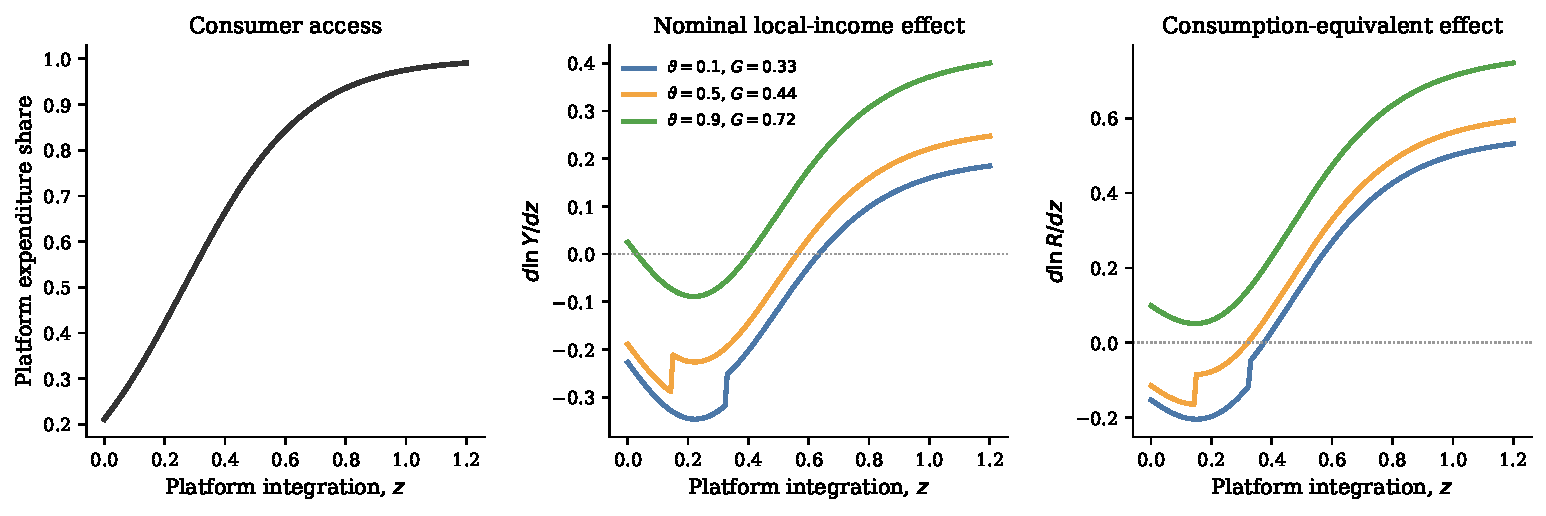
\includegraphics[width=\textwidth]{../figures/figure_3_reform_paths.pdf}
\caption{Event-aware platform-integration and local-income paths}
\label{fig:reform}
\end{figure}

The vertical jumps are economic features of the representative-industry
baseline, not insufficient plot resolution.  Crossing \(G_E\) adds the
candidate industry's entire first-round income, while crossing \(G_L\)
changes the location of its complementary-service payments.  Their numerical
size depends on the standardized ratio of candidate-industry demand to
background income and is not an empirical effect size.  A continuum of
heterogeneous firms would distribute the entry and organization cutoffs and
thereby smooth aggregate income paths, but it would add a productivity
distribution and would remove the closed-form representative-industry
benchmark.  Applying a spline to the present model would instead be
incorrect because it would fabricate intermediate equilibria.

Platform penetration rises for every region.  At low participation, the
candidate industry enters through \(P\) around \(z=0.52\), reversing the
pre-entry decline in both income paths; it switches to \(L\) only near
\(z=0.98\).  At middle participation, entry occurs earlier, around
\(z=0.46\); consumption-equivalent income begins rising at entry, while
nominal income reaches its local minimum around \(z=0.52\), and local
embeddedness occurs near \(z=0.92\).  At high participation, entry occurs
almost immediately, around \(z=0.02\), and the producer switches to \(L\)
around \(z=0.49\).  Before that switch, consumer-side capture drag can keep
the nominal path gently declining; the discrete increase at the switch is the
endogenous local-service and payment-incidence effect.  The consumer platform
share is common across cases because
the baseline state intervention changes producer infrastructure, not the
consumer platform price.

The implied government-participation thresholds at \(z=0.5,c=0.9\) are:
\[
\vartheta_E=\vartheta_R=0.2331,\quad
\vartheta_Y=0.8308,\quad
\vartheta_L=0.9863.
\]
Thus the revised parameterization makes every structural threshold interior
to the admissible participation interval rather than mechanically assigning
most of them a zero state-participation requirement.

The appendix reports six mechanism checks.  Setting
\(\ell_A=\ell_P\) eliminates consumer-side capture drag.  Equating
\(\rho_P\) and \(\rho_L\) eliminates the producer-side spatial payment
difference.  A positive \(\chi^{\mathrm{ext}}\) adds, rather than removes, an
infrastructure--platform complementarity to the parsimonious baseline.  A
positive \(\lambda\) partially localizes platform services.  The reverse case
\(\ell_P>\ell_A\) turns capture drag into a local retention gain.  Finally, an
equal-localization comparison shows that an external-channel restriction and
facilitation have different consumer-access and marginal-entry consequences.
Every figure is generated from the same public code and is accompanied by CSV
source data.

\section{Discussion and Testable Implications}

\subsection{What the model does and does not call development}

The model distinguishes three outcomes.  \(P_M\) measures consumer access.
\(Y\) measures nominal local income generated within the focal accounting
boundary.  \(R\) measures how much market-good consumption that nominal
income can support after the platform price change.  None is a national
welfare measure.  A payment to an external domestic platform is a leakage
from the focal region but remains income somewhere in the national economy.
Likewise, a high local-retention rate is not itself a sufficient policy
objective: a policy can mechanically raise retention by making an efficient
external channel more costly.

This distinction prevents a protectionist reading of the access--capture
problem.  A region with little infrastructure may receive a genuine consumer gain
even when nominal local income falls.  The relevant development question is
not how to preserve every incumbent local intermediary.  It is how to enable
industries consistent with the region's latent comparative advantage to
enter, expand, and build complementary local services without sacrificing the
consumer gains from national integration.

\subsection{Testable implications}

Although the paper contains no original data, its mechanisms generate
specific empirical predictions.

First, platform expansion should reduce consumer price dispersion more
broadly than it increases local producer income.  Consumer effects should
depend primarily on pre-platform access and platform adoption, whereas
producer-income effects should load on the interaction between pre-existing
endowment--industry congruence and infrastructure.  This prediction sharpens
the access--income divergence documented by
\citet{CoutureFaberGuLiu2021}.

Second, among locations with similar platform access, lower
endowment-conditioned relative production costs should predict earlier
seller entry.  Infrastructure should have larger producer effects in
industries that are intensive in locally abundant factors.  A credible test
would construct LCA from pre-shock regional endowments and national industry
factor intensities, rather than infer comparative advantage from post-shock
sales.

Third, producer entry and local capture should not be treated as the same
outcome.  In the platform-dependent region, local seller sales can rise while
platform, settlement, fulfillment, certification, and marketing payments
remain external.  Crossing the embeddedness threshold predicts a discrete
increase in local complementary-service establishments, employment, or
payroll relative to sales.  Buyer--seller locations alone are therefore
insufficient to measure capture; service-provider and ownership locations are
also needed.

Fourth, facilitating infrastructure and an external-channel restriction
should have different joint signatures.  Facilitation should raise outbound
seller participation without raising the local consumer platform price.  An
external-channel restriction may increase the local share of some services
while reducing platform adoption, raising consumer prices, and deterring
marginal platform-dependent sellers.
Empirically similar local-sales shares can therefore conceal very different
access and productivity consequences.

Fifth, partial localization of platform services should compress the
difference between \(P\) and \(L\).  Regions hosting fulfillment, seller
operations, payment, or platform-service employment should retain more value
for a given volume of platform trade.  This prediction separates the location
of production from the location of organizational capture.

\subsection{Scope and extensions}

Several mechanisms are intentionally absent.  Firm heterogeneity would turn
the two organization thresholds into productivity cutoffs, as in trade
intermediation models, but is not needed for the regional thresholds derived
here.  New Economic Geography feedback could make local service depth and
market access endogenous to entry, possibly generating multiple equilibria.
Dynamic endowment accumulation could move a region across industries over
time.  Platform strategic pricing could make the consumer and producer wedges
jointly endogenous.  These are natural extensions, but adding them to the
present paper would obscure its distinct result: platform access can be
diffuse while production and organizational capture remain structurally
conditional.

\section{Conclusion}

Platform integration changes both sides of a local economy.  It improves what
households can buy, and it expands what local producers might sell.  Those
opportunities do not automatically become local development.  Endowments
determine latent comparative advantage; infrastructure determines whether
an industry consistent with that advantage can cover its actual transaction
and fixed costs and enter; and organizational choice determines whether
complementary-service payments remain local.

This chain produces a platform-dependent intermediate state in which local
production exists but organizational capture remains external.  It also
produces separate thresholds for nominal and consumption-equivalent local
income.  Consumer price gains make the real-income threshold weakly lower,
while discrete entry or organization switches explain why strict ordering is
conditional rather than universal.  A facilitating state can help a
potentially viable industry cross these thresholds by relaxing shared
infrastructure financing constraints.  A narrow external-channel restriction
can also induce localization, but only by degrading an outside option and
therefore cannot be treated as equivalent to cost-reducing facilitation.

The central conclusion is consequently not that platforms either help or
hurt local development.  It is that access and capture are different
equilibrium objects.  A common platform can equalize consumer access while
leaving the production and organizational foundations of local income highly
unequal.

\clearpage
\bibliographystyle{apalike}
\bibliography{references}

\clearpage
\appendix
\section{Proofs}

\subsection{Consumer access and channel retention}

\begin{lemma}[Consumer access]
\label{lem:consumer}
Under equations \eqref{eq:consumer_ces} and \eqref{eq:platform_price},
\[
s'(z)=(\eta-1)s(z)[1-s(z)]>0
\quad\text{and}\quad
\frac{d\ln P_M(z)}{dz}=-s(z)<0.
\]
If \(\ell_A>\ell_P\), then \(\omega_C'(z)<0\) and
\(\Lambda(z)>0\).
\end{lemma}

\begin{proof}
Write:
\[
x(z)=a_Pp_P(z)^{1-\eta},
\qquad
a=(1-a_P)p_A^{1-\eta}.
\]
Then \(s=x/(a+x)\).  Because \(d\ln p_P/dz=-1\),
\[
\frac{x'(z)}{x(z)}=-(1-\eta)=\eta-1.
\]
Therefore:
\[
s'
=\frac{x'a}{(a+x)^2}
=(\eta-1)\frac{x}{a+x}\frac{a}{a+x}
=(\eta-1)s(1-s)>0.
\]
For the price index:
\[
\ln P_M=\frac{1}{1-\eta}\ln(a+x).
\]
Hence:
\[
\frac{d\ln P_M}{dz}
=\frac{1}{1-\eta}\frac{x'}{a+x}
=\frac{\eta-1}{1-\eta}s
=-s.
\]
Finally:
\[
\omega_C'(z)=(\ell_P-\ell_A)s'(z).
\]
It is negative when \(\ell_A>\ell_P\).  Since \(D>0\), the definition in
equation~\eqref{eq:capture_drag} then implies \(\Lambda>0\).
\end{proof}

At the limits \(s\rightarrow0\) and \(s\rightarrow1\), \(s'\rightarrow0\).
The platform continues to reduce \(P_M\), but the expenditure-reallocation
margin vanishes at either channel boundary.  This is why capture drag is
largest at an intermediate platform share rather than at complete platform
penetration.

\subsection{Endowment-conditioned production costs}

The background technology in equation~\eqref{eq:background_technology}
implies:
\[
w_i=(1-\theta_0)\frac{Y_{i0}}{L_i},
\qquad
r_i=\theta_0\frac{Y_{i0}}{K_i}.
\]
With \(Y_{i0}=A_0K_i^{\theta_0}L_i^{1-\theta_0}\), division by the relevant
factor endowment yields equation~\eqref{eq:factor_prices}.  Substituting those
factor prices into the candidate industry's Cobb--Douglas unit expenditure
function gives:
\begin{align*}
c^P_{ij}
&=
\frac{1}{A_j}
\left(\frac{\theta_0A_0e_i^{\theta_0-1}}{\theta_j}\right)^{\theta_j}
\left(
\frac{(1-\theta_0)A_0e_i^{\theta_0}}{1-\theta_j}
\right)^{1-\theta_j}\\
&=
\frac{A_0}{A_j}
\left(\frac{\theta_0}{\theta_j}\right)^{\theta_j}
\left(\frac{1-\theta_0}{1-\theta_j}\right)^{1-\theta_j}
e_i^{\theta_0-\theta_j}\\
&\equiv \xi_j e_i^{\theta_0-\theta_j}.
\end{align*}
Thus:
\[
\frac{\partial\ln c^P_{ij}}{\partial\ln e_i}
=\theta_0-\theta_j.
\]
For \(\theta_j>\theta_0\), capital abundance lowers the candidate industry's
production cost relative to the background opportunity cost.  LCA still
requires the external-reference double ratio in equation~\eqref{eq:lca};
the derivative is only the local structural component of that comparison.

\subsection{Proof of Proposition~\ref{prop:entry}}

\begin{proof}
For a given organization \(r\), equation~\eqref{eq:revenue_profit} becomes:
\[
\pi_r(z,G)
=
k\Mcal_0e^{\varepsilon z+\Omega(z)G}(c+d_r)^{1-\sigma}
-F_r.
\]
It is strictly increasing in \(G\) whenever \(\Omega(z)>0\).  The unique raw
zero-profit threshold is equation~\eqref{eq:mode_entry_threshold}.  Direct
differentiation gives:
\[
\frac{\partial G_r^0}{\partial c}
=
\frac{\sigma-1}{\Omega(z)(c+d_r)}>0.
\]
The minimum of two strictly increasing functions is strictly increasing:
for \(c_2>c_1\), both \(G_P^0(c_2)>G_P^0(c_1)\) and
\(G_L^0(c_2)>G_L^0(c_1)\), so their minimum at \(c_2\) exceeds their minimum
at \(c_1\).  The truncation at zero preserves weak monotonicity.  At an
interior threshold, the relationship is strict.

Holding the external-region and background-industry ratios fixed,
\(\partial c/\partial\mathcal C^P_{ij}>0\).  The chain rule therefore gives:
\[
\frac{\partial G_E}{\partial\mathcal C^P_{ij}}
=
\frac{\partial G_E}{\partial c}
\frac{\partial c}{\partial\mathcal C^P_{ij}}>0
\]
at an interior threshold.

For the ACA interpretation, the focal region's delivered marginal cost is
\(\tau_O(z,G)(c+d_r)\).  Since
\[
\frac{\partial\ln\tau_O(z,G)}{\partial G}
=-(\gamma+\chi z)<0,
\]
infrastructure lowers the focal region's total-cost ratio relative to a fixed
reference region.  Stronger LCA starts from a lower production-cost ratio, so
it requires weakly less \(G\) both to achieve a total-cost advantage and to
cover the fixed cost.  The first condition is ACA; the second is viability.
Entry and sales are realization.
\end{proof}

\section{Complete Entry and Organization Classification}

Let:
\[
b_P=k(c+d_P)^{1-\sigma},
\qquad
b_L=k(c+d_L)^{1-\sigma},
\]
so \(b_L>b_P>0\).  It is convenient to express the state problem in terms of
effective market scale:
\[
X(z,G)=\Mcal_0e^{\varepsilon z+\Omega(z)G}.
\]
Profits are:
\[
\pi_P=Xb_P-f,
\qquad
\pi_L=Xb_L-f-F.
\]
The corresponding market-scale thresholds are:
\[
X_P=\frac{f}{b_P},
\qquad
X_{L0}=\frac{f+F}{b_L},
\qquad
X_X=\frac{F}{b_L-b_P}.
\]

\begin{lemma}[Three-region condition]
\label{lem:three_region}
Define:
\[
\bar F=f\frac{b_L-b_P}{b_P}.
\]
If \(F>\bar F\), then:
\[
X_P<X_{L0}<X_X,
\]
equivalently \(G_P^0<G_L^0<G_X\), and the equilibrium states are:
\[
\begin{cases}
0,&X<X_P,\\
P,&X_P\leq X<X_X,\\
L,&X\geq X_X.
\end{cases}
\]
If \(F=\bar F\), all three thresholds coincide.  If \(F<\bar F\), the
platform-dependent interval is absent and the producer enters through \(L\).
\end{lemma}

\begin{proof}
First:
\begin{align*}
X_P<X_{L0}
&\Longleftrightarrow
\frac{f}{b_P}<\frac{f+F}{b_L}\\
&\Longleftrightarrow
f(b_L-b_P)<Fb_P\\
&\Longleftrightarrow F>\bar F.
\end{align*}
Second:
\begin{align*}
X_{L0}<X_X
&\Longleftrightarrow
\frac{f+F}{b_L}<\frac{F}{b_L-b_P}\\
&\Longleftrightarrow
f(b_L-b_P)<Fb_P\\
&\Longleftrightarrow F>\bar F.
\end{align*}
Thus the same condition orders all three thresholds.  Below \(X_P\), both
profits are negative.  At \(X_P\), \(\pi_P=0\), while:
\[
\pi_L-\pi_P
=X_P(b_L-b_P)-F
=\bar F-F<0.
\]
Because:
\[
\pi_L-\pi_P=X(b_L-b_P)-F
\]
is strictly increasing in \(X\), it crosses zero exactly once at \(X_X\).
This proves the three states.  Equality collapses all thresholds to one
point.  If \(F<\bar F\), the local mode is already more profitable at the
first viable entry scale, so \(P\) is never selected.
\end{proof}

\section{Proof of Proposition~\ref{prop:embedding}}

\begin{proof}
Define:
\[
\Delta(c)
=(c+d_L)^{1-\sigma}-(c+d_P)^{1-\sigma}>0.
\]
The raw switch threshold is:
\[
G_X
=
\frac{\ln F-\ln[k\Mcal_0e^{\varepsilon z}]-\ln\Delta(c)}
{\Omega(z)}.
\]
Its cost derivative is:
\[
\frac{\partial G_X}{\partial c}
=-\frac{\Delta'(c)}{\Omega(z)\Delta(c)}.
\]
Because:
\[
\Delta'(c)
=(1-\sigma)
\left[(c+d_L)^{-\sigma}-(c+d_P)^{-\sigma}\right]<0,
\]
we have \(\partial G_X/\partial c>0\).  Truncation at zero preserves weak
monotonicity.  The LCA result follows from
\(\partial c/\partial\mathcal C^P_{ij}>0\).

For \(G>G_X\):
\[
\pi_L-\pi_P
=
k\Mcal_0e^{\varepsilon z+\Omega G}\Delta(c)-F>0.
\]
Hence \(L\) is selected whenever it also weakly dominates no entry; the
classification in Lemma~\ref{lem:three_region} covers the possible entry
orders.

Since \(d_L<d_P\):
\[
(c+d_L)^{1-\sigma}>(c+d_P)^{1-\sigma},
\]
and therefore \(\Rcal_L>\Rcal_P\) at a common \((z,G)\).  The payment-flow
definitions imply:
\[
\rho_L=1>
1-\frac{d_P}{\mu(c+d_P)}
=\rho_P.
\]
Both inequalities are strict, so:
\[
B_j^L=\rho_L\Rcal_L
>
\rho_P\Rcal_P=B_j^P.
\]
The external payment changes from \(d_Pq_P>0\) to zero in the polar baseline,
while the unit organizational service \(d_Lq_L\) and the shared fixed
organizational service \(F\) are locally supplied.  The organizational switch
therefore changes local service income, external payments, and total
first-round local income.
\end{proof}

\section{Proof of Proposition~\ref{prop:income_thresholds}}

\subsection{Income derivatives within a producer state}

Fix an active producer organization \(r\).  The local producer-income term can
be written:
\[
B_j^r(z,G)
=
A_r
\exp\{\varepsilon z+\Omega(z)G\},
\]
where:
\[
A_r
=
\rho_r\Mcal_0\mu^{1-\sigma}(c+d_r)^{1-\sigma}>0.
\]
Therefore:
\[
\frac{\partial\ln B_j^r}{\partial G}
=\Omega(z)>0,
\]
and:
\[
\frac{\partial\theta_r}{\partial G}
=
\Omega(z)\theta_r(1-\theta_r)>0.
\]
Define:
\[
a(G)=\varepsilon+(\sigma-1)\chi G\geq0.
\]
The nominal integration effect within organization \(r\) is:
\[
h_Y(G)=\theta_r(G)a(G)-\Lambda(z).
\]
Its derivative is:
\begin{equation}
h_Y'(G)
=
\Omega(z)\theta_r(1-\theta_r)a(G)
+\theta_r(\sigma-1)\chi>0.
\label{eq:nominal_effect_derivative}
\end{equation}
The price term \(\alpha_Ms(z)\) is independent of \(G\), so:
\[
h_R'(G)=h_Y'(G)>0
\]
within an active state.  In the no-entry state, \(\theta=0\); both effects
are constant in \(G\) until entry.

\subsection{Jumps at state changes}

Immediately before entry, \(\theta=0\), so \(h_Y=-\Lambda\).  Immediately
after entry, the viable mode generates positive sales and local producer
income, so \(\theta>0\).  Since \(a(G)\geq0\), the integration effect jumps
weakly upward and strictly upward if \(a(G)>0\).

At a \(P\)-to-\(L\) switch, Proposition~\ref{prop:embedding} gives
\(B_j^L>B_j^P\).  Hence \(\theta_L>\theta_P\), while \(a(G)\) and
\(\Lambda(z)\) are unchanged at the switch.  Both nominal and real effects
jump strictly upward.

\subsection{Existence, uniqueness, and ordering}

\begin{proof}[Completion of the proof]
The preceding derivatives and jump results imply that the integration effects
are globally nondecreasing in \(G\), strictly increasing in every active
organization, and have no downward state jumps.  Under the baseline
\(\ell_A>\ell_P\) and an interior platform share, the no-entry effect is
strictly negative because \(\Lambda>0\).

As \(G\rightarrow\infty\), the local mode is selected,
\(\theta_L\rightarrow1\), and:
\[
a(G)=\varepsilon+(\sigma-1)\chi G\rightarrow\infty
\]
when \(\chi>0\).  Hence \(h_Y(G)\rightarrow\infty\), and the real effect is
larger still.  More generally, it is sufficient to assume a finite upper
endpoint at which the relevant effect is positive.  Monotonicity and endpoint
crossing therefore imply a unique minimum threshold, allowing the crossing to
occur either continuously or at an upward jump.

Pointwise:
\[
h_R(G)=h_Y(G)+\alpha_Ms(z)>h_Y(G).
\]
Thus every \(G\) that makes the nominal effect nonnegative also makes the real
effect positive, establishing \(G_R\leq G_Y\).

Suppose both roots lie in the same active continuous organization and are
interior.  At \(G_Y\), \(h_Y(G_Y)=0\), so:
\[
h_R(G_Y)=\alpha_Ms(z)>0.
\]
Since \(h_R\) is continuous and strictly increasing in that organization, its
zero must occur strictly below \(G_Y\).  Hence \(G_R<G_Y\).  If both effects
jump from negative to nonnegative at the same discrete state change, their
minimum thresholds are identical even though \(h_R>h_Y\) on either side.

It remains to establish the comparative static with respect to LCA.  For the
local mode:
\[
B_j^L
=
\Mcal\mu^{1-\sigma}(c+d_L)^{1-\sigma},
\]
which is strictly decreasing in \(c\).  For the platform mode:
\begin{align*}
B_j^P
&=
\Mcal\mu^{1-\sigma}
\left[
(c+d_P)^{1-\sigma}
-\frac{d_P}{\mu}(c+d_P)^{-\sigma}
\right].
\end{align*}
Differentiating the bracket gives:
\begin{align*}
&(1-\sigma)(c+d_P)^{-\sigma}
+\frac{\sigma d_P}{\mu}(c+d_P)^{-\sigma-1}\\
&\qquad
=-(\sigma-1)c(c+d_P)^{-\sigma-1}<0,
\end{align*}
where \(\mu=\sigma/(\sigma-1)\).  Thus lower \(c\) raises local producer
income in either mode.  It also weakly advances entry and the switch to the
higher-income local mode by Propositions~\ref{prop:entry} and
\ref{prop:embedding}.  At every fixed \(G\), stronger LCA therefore weakly
raises \(\theta_{r^*}\) and the two integration effects.  Their minimum
thresholds weakly fall.  The relationship is strict when the relevant root
remains interior to the same active organizational state.
\end{proof}

\section{Proof of Proposition~\ref{prop:state}}

\begin{proof}
Define the infrastructure provider's first-order condition:
\[
\Phi(G,\vartheta)
=
\mathcal U_I'(G)-\kappa_I(\vartheta)C'(G)=0.
\]
Its derivative with respect to \(G\) is:
\[
\Phi_G
=
\mathcal U_I''(G)-\kappa_I(\vartheta)C''(G)<0.
\]
The objective is therefore strictly concave and has at most one interior
solution.  Under the maintained endpoint conditions, that solution exists and
is unique.  Since:
\[
\Phi_\vartheta
=-\kappa_I'(\vartheta)C'(G)>0,
\]
implicit differentiation gives:
\[
G'(\vartheta)
=-\frac{\Phi_\vartheta}{\Phi_G}>0.
\]

For any fixed structural threshold \(G_H\), the monotonicity of
\(G(\vartheta)\) implies that the set
\(\{\vartheta:G(\vartheta)\geq G_H\}\) is an interval.  When nonempty, it has
a unique minimum \(\vartheta_H\), except for an economically irrelevant flat
boundary if the infrastructure solution itself is constrained.  Increasing
\(\vartheta\) reduces \(G_H-G(\vartheta)\).  Stronger LCA lowers
\(G_E,G_L,G_R,G_Y\) by Propositions~\ref{prop:entry}--\ref{prop:income_thresholds};
applying the increasing inverse of \(G(\vartheta)\) weakly lowers the
associated participation thresholds.

For the protection comparison, a consumer wedge \(\tau_C>1\) changes the
effective platform price to \(\tau_C\bar p_Pe^{-z}\).  The CES price index is
increasing in an input price, so protection raises \(P_M\) and lowers the
platform expenditure share.  On the producer side:
\[
\frac{\partial G_P^0}{\partial d_P}
=
\frac{\sigma-1}{\Omega(z)(c+d_P)}>0.
\]
Thus protection makes the low-fixed-cost external entry mode harder for a
marginal producer.

Let:
\[
\Delta=(c+d_L)^{1-\sigma}-(c+d_P)^{1-\sigma}.
\]
Because:
\[
\frac{\partial\Delta}{\partial d_P}
=
(\sigma-1)(c+d_P)^{-\sigma}>0,
\]
the switch threshold satisfies:
\[
\frac{\partial G_X}{\partial d_P}
=
-\frac{1}{\Omega(z)\Delta}
\frac{\partial\Delta}{\partial d_P}<0.
\]
Protection can therefore induce a switch toward \(L\), but it does so by
worsening \(P\), while simultaneously harming consumer access and making
platform-based entry more difficult.  Facilitation raises \(G\), which
increases market access under both modes and does not enter the consumer price
equation.  The policies are not equivalent.
\end{proof}

\section{Boundary Cases and Counterexamples}

\subsection{No consumer-side capture gap}

If \(\ell_A=\ell_P\), then:
\[
\omega_C(z)=\ell_A,
\qquad
\Lambda(z)=0.
\]
The nominal effect becomes:
\[
\frac{d\ln Y}{dz}
=
\theta_r[\varepsilon+(\sigma-1)\chi G]\geq0
\]
in every active producer state.  A negative nominal effect can then arise
only in an extension with another first-round loss.  This case confirms that
the baseline negative region is generated by an explicit payment-incidence
gap rather than platform terminology.

If \(\ell_P>\ell_A\), then \(\Lambda<0\).  Platform substitution raises
consumer-side retention as well as reducing the price index.  Both nominal
and real effects shift upward; the low-infrastructure loss region may vanish.

\subsection{No producer-side spatial payment gap}

Setting \(\lambda=1\) in equation~\eqref{eq:partial_localization} gives
\(\rho_P=1=\rho_L\).  The organization switch can still raise sales because
\(d_L<d_P\), but it no longer changes the spatial retention rate.  This case
separates the cost advantage of local organization from its payment-location
advantage.

\subsection{No infrastructure--platform complementarity}

If \(\chi=0\), producer market access is:
\[
\Mcal(z,G)
=
\Mcal_0e^{\varepsilon z+(\sigma-1)\gamma G}.
\]
Infrastructure can still raise the level of candidate-industry income and
therefore \(\theta_r\), but it no longer increases the marginal producer
benefit of platform integration directly.  Equation~\eqref{eq:nominal_effect}
loses the term \((\sigma-1)\chi G\).  The threshold mechanism can survive,
but the strong complementarity interpretation cannot.

\subsection{Collapse of the platform-dependent region}

Lemma~\ref{lem:three_region} gives the exact counterexample to a universal
three-stage development path.  When \(F\leq\bar F\), the local mode is
sufficiently inexpensive in fixed-cost terms that the candidate industry
enters directly through \(L\).  Platform dependence is therefore neither
necessary nor universal.

\subsection{Weak rather than strict income-threshold ordering}

Suppose an entry or organizational switch occurs at \(\widehat G\), with:
\[
h_R(\widehat G^-)<0,\qquad h_Y(\widehat G^-)<0,
\]
and:
\[
h_R(\widehat G^+)\geq0,\qquad h_Y(\widehat G^+)\geq0.
\]
Then:
\[
G_R=G_Y=\widehat G.
\]
The pointwise inequality \(h_R>h_Y\) is not enough to create two different
minimum thresholds when a common discrete jump crosses both zeroes.  This is
why Proposition~\ref{prop:income_thresholds} states strict ordering only under
a continuous interior-root condition.

\subsection{Instability of the local-income closure}

If:
\[
D(z)=1-\beta-\alpha_M\omega_C(z)\leq0,
\]
the household-spending recursion does not converge.  This is not an
alternative equilibrium of the paper.  It is an inadmissible parameter
region.  The baseline values satisfy \(D(z)>0\) for the full numerical
support.

\section{Mapping to the Companion EL Income Block}

The companion access--capture model can be written:
\[
Y^{EL}
=
\frac{B^{EL}+\omega^{EL}G^{EL}}
{1-\beta^{EL}-\alpha^{EL}\omega^{EL}}.
\]
The present paper does not insert this expression into the producer problem.
It uses the following one-to-one mapping only after first-round payments have
been determined:

\begin{table}[htbp]
\centering
\caption{Mapping to the companion income-propagation block}
\begin{tabular}{p{0.28\textwidth}p{0.29\textwidth}p{0.35\textwidth}}
\toprule
Companion object & Present object & Accounting rule\\
\midrule
\(B^{EL}+\omega^{EL}G^{EL}\)
& \(B_0+B_j^{r^*}\)
& autonomous first-round local income only\\
\(\alpha^{EL}\)
& \(\alpha_M\)
& household market-good expenditure share\\
\(\beta^{EL}\)
& \(\beta\)
& locally supplied nontraded-good expenditure share\\
\(\omega^{EL}\)
& \(\omega_C(z)\)
& local income content of induced market-good spending\\
consumer price index
& \(P_M(z)\)
& identical CES market-good price concept\\
nominal income
& \(Y\)
& equation~\eqref{eq:nominal_income}\\
consumption-equivalent income
& \(R\)
& equation~\eqref{eq:real_income}\\
\bottomrule
\end{tabular}
\end{table}

The candidate-industry sales payment enters \(B_j^{r^*}\) once.  It does not
also enter \(\omega_C\), which applies only to subsequent household
market-good expenditure.  The external platform organization payment enters
\(\rho_P\) once.  Consumer-channel external payments enter \(\ell_P\) and
\(\omega_C\), not \(\rho_P\).  This separation prevents production,
organizational services, and induced household spending from being counted
twice.

\section{Numerical Reproducibility and Mechanism Closures}

The numerical implementation consists of:
\begin{itemize}
 \item \texttt{code/numerical/model.py}, which implements the equations and
 equilibrium choices;
 \item \texttt{code/numerical/generate\_figures.py}, which generates all
 figures and source-data CSV files;
 \item the validation script, which checks analytical derivatives, finite
 differences, threshold uniqueness, the three-region condition, boundary
 cases, and state monotonicity.
\end{itemize}

For \(z=0.5,c=0.8\), the code obtains:
\[
G_P^0=-0.070176,\quad
G_L^0=0.126129,\quad
G_X=0.256065,
\]
\[
G_R=0.046348,\quad
G_Y=0.550487.
\]
Finite-difference derivatives have the signs established in the proofs.
The program also verifies that lowering \(F\) below \(\bar F\) removes the
platform-dependent interval and that equal consumer-channel local contents
set \(\Lambda\) exactly to zero.

The file
\texttt{figures/source\_data/appendix\_mechanism\_closures.csv}
reports the full \(G\)-grid for:
\begin{enumerate}
 \item the baseline;
 \item \(\ell_A=\ell_P\);
 \item complete platform-service localization;
 \item \(\chi=0\);
 \item partial platform-service localization.
\end{enumerate}
All reported exercises use normalized, illustrative values.  No parameter is
estimated, and the exercises do not constitute a calibration.


\end{document}
